\section{Methods}\label{sec:methods}

\subsection{Genome-Scale Models}\label{ssec:genome_scale_models}

% \begin{itemize}
%  \item How are they created?
%  \begin{itemize}
%   \item genome or annotated genome are automatically translated to a GEM
%   \item tools: Pathway Tools \cite{karp2009pathway}, SEED \cite{henry2010high}
%   \item AUTOGRAPH \cite{notebaart2006accelerating} which reuses existing models
%   \item \cite{santos_practical_2011}
%   \item must be refined by hand
%   \item ``too many important organism-specific choices''
%   \item ``omissions, wrong assignments and gaps, and inconsistencies''
%   \item biomass function
%   \item input/output reactions
%   \item ``gene-to-protein-to-reaction (GPR) association that describes the genetic basis for a
% metabolic reaction ''
%   \item A reconstruction collects all the available
% biochemical, genetic, and genomic (BiGG) information that is available on a cellular
% process of interest, and then organizes it in a formal, mathematical fashion that is
% consistent with the corresponding fundamental chemical and genetic properties
%   \item \cite{palsson2015systems}
%   \item Networks are composed of compounds (nodes) and reactions (links)
%   \item Such mathematical
% representation is based on the stoichiometric coefficients that count the molecules that
% are consumed and produced by a biochemical reaction.
%   \item It is important to note that a map for a network can be drawn in many
% different ways, but the mathematical representation is unique.
%   \item Ultimately, a reconstruction can reach a genome-scale when all the known
% biochemical and genetic processes that are found on a genome are accounted for
%   \item they now include the details of both protein
% synthesis and structure, transcriptional regulation, and other processes
%   \item A network reconstruc-
% tion is the basis for a computational model for network states (i.e., phenotypic states)
%  \end{itemize}
% 
%  \item What does they contain?
%  \item What is missing?
% \end{itemize}

A genome-scale model (GEM) is an analytical reconstruction of ideally all cellular process of a cell.
All available biochemical, genetic and genomic (BiGG) information of the processes are analyzed to
identify gene-to-protein-to-reaction (GPR) associations and involved compounds. 
Based on this data a network composed of compounds (nodes) and reactions (links) is created and added
to the reconstruction.
\cite{palsson2015systems}

Tools like \textit{Pathway Tools}\cite{karp2009pathway},
\textit{SEED}\cite{henry2010high} or \textit{AUTOGRAPH}\cite{notebaart2006accelerating} are used to
generate a reconstruction based on a (annotated) genome. The produced models contain many
wrong assignments, gaps and inconsistencies due to many organism-specific choices and must be refined by hand.
A biomass function to model growth and input/output reactions are added to
the network\cite{santos_practical_2011}.

The reconstruction is the basis to create geno- and phenotypes of a cell and to transform it into
mathematical models for further analysis.
An important mathematical representation is the stoichiometric matrix. It uniquely represents the metabolic
network of the cell, based on the stoichiometric constants of its reactions\cite{palsson2015systems}.

\begin{figure}[!h]
\centering
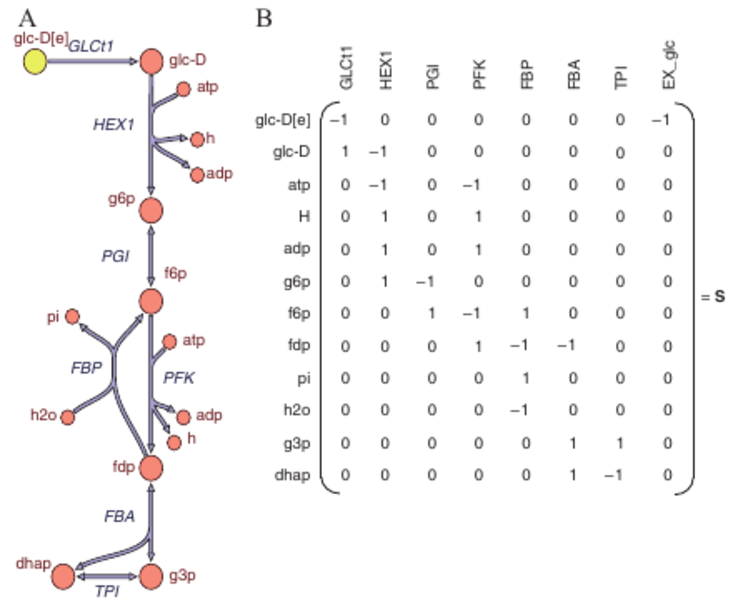
\includegraphics[width=\linewidth]{figures/Selection_011.pdf}
\caption{(create simplified version here, combine with figure \ref{fig:reconstruction_GPR_example})}
\label{fig:reconstruction_to_matrix_example}
\end{figure}

\begin{figure}[!h]
\centering
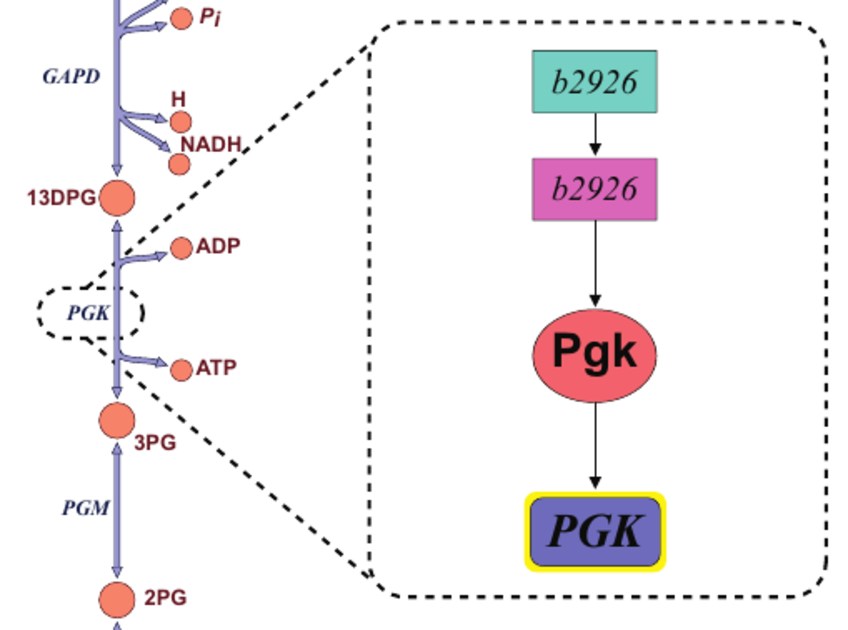
\includegraphics[width=\linewidth]{figures/Selection_013.pdf}
\caption{(create simplified version here, combine with figure \ref{fig:reconstruction_to_matrix_example})}
\label{fig:reconstruction_GPR_example}
\end{figure}

\subsection{Flux Balance Analysis}\label{ssec:flux_balance_analysis}

Flux Balance Analysis (FBA) is a mathematical tool which analysis possible flux
distributions through the metabolic network based on the stochiometric matrix of 
a GEM.

The system of linear equations built by the stoichiometric matrix $S$ of a GEM is
usually underdetermined. To choose one flux distribution from the solution space
spanned by $S$, it is assumed the organism adapted its metabolic fluxes to a certain
environment and is now in a steady state where the fluxes are optimal distributed
recording to some goal. In FBA this flux distribution is chosen by solving a
optimization problem as in equation \ref{eq:fba_optimization_formula} using linear
programming (LP) \cite{orth_what_2010}.

\begin{equation}\label{eq:fba_optimization_formula}
\begin{aligned}
& \underset{\bm{v}}{\text{max}}
& & a = \bm{w}^T \bm{v} \\
& \text{s.t.}
& & S\bm{v} = \bm{0}, \\
&&& \bm{v_{min}} \leq \bm{v} \leq \bm{v_{max}}
\end{aligned}
\end{equation}

The fluxes in the metabolic network $\bm{v}$ are optimized so that $a$ is maximized
where $\bm{w}$ is a weighting vector which defines the adaption goal of the cell.
A often used goal is to maximize the growth of the organism.
The optimization is done using mostly two constraints, (1) the stoichiometric constants $S$
for each reaction which is defined by the used GEM and (2) lower and upper bounds for 
each flux, $\bm{v_{min}}$ and $\bm{v_{max}}$, in the metabolic network but further 
constraints can be added as well.

The lower and upper bounds can be used to simulate gene know-outs by setting the upper
bound of reactions dependent on this gene to zero or to define environmental conditions
like the availability of certain metabolites.

The chosen solution by the LP solver represents a phenotype of the given organism
due to adaption to its environment but FBA has its limitations. Usually GEMs does
not model regulatory structures as activation of enzymes or regulation of gene
expressions. As the GEM does not contain kinetic parameters of the involved compounds, 
their densities can not be considered and must be modeled externally \cite{orth_what_2010}.

% \begin{itemize}
%   \item Sort introduction
%   \begin{itemize}
%     \item tool to study biochemical networks
%     \item ``calculates the flow of metabolites through
% this metabolic network''
%   \end{itemize}
%   \item What is the basic problem?
%   \begin{itemize}
%    \item stochiometric matrix can not be solved uniquely
%   \end{itemize}
%   \item How does FBA work?
%   \begin{itemize}
%     \item ``Mathematically, an
% ‘objective function’ is used to quantitatively
% define how much each reaction contributes
% to the phenotype.''
%     \item ``define a system of linear
% equations``
%     \item ''In flux balance analysis, these
% equations are solved using linear program-
% ming``
%     \item ``Every reaction can also be given
% upper and lower bounds''
%     \item ``These balances and bounds
% define the space of allowable flux distribu-
% tions of a system''
%     \item  ``To change the environmental
% conditions (such as substrate availabil-
% ity), we change the bounds on exchange
% reactions (that is, reactions representing
% metabolites flowing into and out of the sys-
% tem)``
%     \item ''Nonzero lower bounds can also
% force a minimal flux through artificial reac-
% tions [...] to sim-
% ulate energy demands not associated with
% growth``
%     \item ''Constraints can even be used to
% simulate gene knockouts by limiting reac-
% tions to zero flux''
%    \item ``Constraints are represented in two ways,
% as equations that balance reaction inputs
% and outputs and as inequalities that impose
% bounds on the system. ''
%    \item ``These stoichiometries impose
% constraints on the flow of metabolites through
% the network.''
%     \item steady state
%     
%   \end{itemize}
%   \item interpretation
%   \begin{itemize}
%     \item FBA results can be seen as phenotypes
%     \item ``FBA is an important tool for harnessing the
% knowledge encoded in these models''
%   \end{itemize}
%   \item ``FBA has limitations''
%   \begin{itemize}
%    \item ``does not use kinetic parameters, it cannot
% predict metabolite concentrations''
%     \item ``only suitable for determining fluxes at steady
% state''
%     \item `` FBA
% does not account for regulatory effects such
% as activation of enzymes by protein kinases
% or regulation of gene expression''
%   \end{itemize}
% 
% \end{itemize}



\subsection{Simulation Algorithm}

\update{
\begin{table}[h]
\centering
\caption{Overview of implemented features compared to DMMM}
\label{tab:overview_implemented_features_compared_to_dmmm}
\begin{tabular}{llllll}
\rowcolor[HTML]{EFEFEF} 
\cellcolor[HTML]{EFEFEF} Feature                  & \cellcolor[HTML]{EFEFEF}DMMM & \cellcolor[HTML]{EFEFEF}This project\\
Model                                    &   &  \\
\hspace{0.5cm}arbitrary many GEMs & yes & yes \\
\hspace{0.5cm}\begin{tabular}[c]{@{}l@{}}arbitrary many metabolites\\ in environment\end{tabular} & yes & yes \\
\hspace{0.5cm}mortablility of bacteria & \begin{tabular}[c]{@{}l@{}}yes\\(in output flux)\end{tabular} & yes \\
\hspace{0.5cm}\begin{tabular}[c]{@{}l@{}}input/output flux of bacteria\\ and metabolites\end{tabular} & yes & no \\
\hspace{0.5cm}\begin{tabular}[c]{@{}l@{}}parameterized initial state\\ of environment composition\end{tabular} & yes & yes \\
\hspace{0.5cm}Michaelis-Menten kinetics & yes & yes \\
Algorithm &  &  \\
\hspace{0.5cm}ODE solver & yes & yes \\
\hspace{0.5cm}different ODE solvers & yes & no \\
\hspace{0.5cm}analytical solver & yes &no \\
\end{tabular}
\end{table}}

As described by Zhuang et al. in \cite{zhuang_genome-scale_2011} the algorithm uses an ODE solver with embedded FBA. An FBA is solved
for each GEM in the model and for each time step in the discretised simulation time interval considering the changed metabolite and
bacteria densities in the shared environment. The results of the FBAs are used by the ODE solver to solve the differential equations

\begin{equation} \label{eq:diff_eq_x}
	\frac{\dd X_M}{\dd t} = (\mu_M - \mathrm{Mort}(\mu_M)) X_M
\end{equation}
\begin{equation} \label{eq:diff_eq_s}
	\frac{\dd S_m}{\dd t} = \displaystyle\sum_{M \in models} v_{M,m} X_M
\end{equation}

which models the dynamics of the bacteria's environment \cite{zhuang_design_2012}. Equation \ref{eq:diff_eq_x} updates
the bacteria masses $X_M$ in the shared medium where $M$ are the bacteria models, $\mu_M$ the growth rate of bacteria $M$ and the function
$\mathrm{Mort}()$ models the mortability of that bacteria dependent on its growth rate.
Equation \ref{eq:diff_eq_s} updates the amount of molecules $S_m$ of metabolites in the shared medium where $v_{M,m}$ are the
output fluxes of metabolite $m$ by bacteria model $M$.

In each time step each bacteria's metabolite intake must be changed dependent on the densities of the metabolites in the shared environment.
To model saturation of metabolite intake for high metabolite densities Zhuang et al. implemented Michaelis-Menten kinetics \cite{johnson2011original}

\begin{equation} \label{eq:michaelis-menten}
% b_{M,m} = \frac{v_{max,M,m} s_m}{s_m + k_{M,m}} \prod_{a=1}^M \frac{1}{1 + \frac{s_a}{\mat{I}_{a,i,j}}}
 b_{M,m} = v_{max,M,m} \; \frac{s_m}{k_{M,m}+s_m} \; \prod_{m'} \cfrac{1}{1+\cfrac{s_{m'}}{I_{M,m,m'}}}
\end{equation}

Formula \ref{eq:michaelis-menten} describes the the dependency of the upper bound of the input flux $b_{M,m}$ for metabolite $m$ of model $M$ on the metabolite density
$s_m$ in the shared medium. The formula is the product of two expressions. The left expression describes the actual dependency
of the intake flux on the metabolite density and is modeled using Michaelis-Menten kinetics where $v_{max,M,m}$ is the maximal
possible input flux and $k_{M,m}$ is the Michaelis-Menten constant. This constant defines the metabolite density where the
input flux is exactly at the half of its maximal possible value. The right expression of formula \ref{eq:michaelis-menten}
models the inhibition of the input flux of metabolite $m$ of bacteria $M$ by another metabolite $m'$ in the shared medium.
This expression can be used to add toxic effects of certain compounds on the metabolism of a bacteria. This therm is defined
by the inhibition constant $I_{M,m,m'}$ which, similar to the Michaelis-Menten constant, defines the metabolite density $s_{m'}$
where the value of this therm is exactly 0.5.

Algorithm \ref{alg:differential_equation_with_embedded_fba} shows a basic implementation of the differential equations solved by an ODE
solver during the simulation similar to DMMM \cite{zhuang_genome-scale_2011}.

\update{
The algorithm expects a list of bacteria models consisting of
\begin{itemize}
 \item GEM of this bacteria: A, $\bm{v_{min}}$, $\bm{v_{max}}$, $\bm{w_{growth}}$
 \item $\bm{v_{mm}}$ (Michaelis-Menten $V_{max}$) for each exchange metabolite and species
 \item $\bm{k}$ (Michaelis-Menten K) for each exchange metabolite and species
 \item mortality $\mu(v_\bio)$
 \item inhibition constants $\mat{I}_a$
\end{itemize}}

Furthermore a list of all exchange metabolites in the environment, the bacteria and metabolite densities.


\begin{algorithm}
	\DontPrintSemicolon
	\def\model{\ensuremath{\mathrm{model}}}
    \KwIn{metabolites in shared medium $m$, bacteria populations $X_M$, metabolite counts $S_m$}
    \KwOut{slope of bacteria masses and amounts metabolite molecules $\dot{X}_M, \dot{S}_m$}
    \KwData{bacteria models $\model_M$, Michaelis-Menten constants of model $M$ $\v{k}_{M}$, inhibition matrices of model $M$  $\mat{I}_{M}$, Total volume $V$}
    
	$\v s \KwAssign \frac{\v S}{V}$\;
	
	\ForEach{model $M$ in models}{
		\ForEach{metabolite $m$ in exchanges of $M$}{
%			$\displaystyle b_{M,m} = v_{max,M,m} \; \frac{s_m}{k_{M,m}+s_m} \; \prod_{m'} \cfrac{1}{1+\cfrac{s_{m'}}{\mat{I}_{M,m,m'}}}$\;
			$b_{M,m} = \mathrm {upper\_bound}(\v{s}, M, m)$
		}
	}
	
% 	$\dot{\v x} \KwAssign [0,\dotsc,0]$\;
% 	$\dot{\v S} \KwAssign [0,\dotsc,0]$\;
	
    \ForEach{Model $M$ in models}{
      $\mu_M, \v{v_M}$ \KwAssign $\mathrm{FBA}(M, \v{b_{M}})$\;
      $\dot{X}_M = (\mu_M - \mathrm{Mort}(\mu_M)) \mul X_M$\;
      $\dot{\v S} = \dot{\v S} + \v{v_M} \mul X_M$\;
    }
      
    
    \Return{$[\dot{\v X},\dot{\v S}]$}
    \caption{Differential equation with embedded FBA}
    \label{alg:differential_equation_with_embedded_fba}
\end{algorithm}

In a first step, the absolute metabolite counts are converted to densities, and all smaller than zero entries are set to zero. This step is necessary since negative densities are unphysical and forbidden, hence the function is transformed as proposed in \cite{shampine_nonneg_2005}.

Next, the lower bounds of the intake fluxes are updated for each bacteria $M$ and exchange metabolite $m$ according to the Michaelis-Menten formula \ref{eq:michaelis-menten}.

\update{
In a further step, the GEMs are optimized for growth using FBA, the results are used as biomass production $\bm{v}_\bio$ and actual input and output
fluxes $\bm{v_j}$ of bacteria j in this time step.
The mortality is considered by subtracting the constants $\bm{\mu}(\v{v}_\bio)$ from the biomass production rates $\bm{v}_\bio$.
The slopes $\dot{\bm{x}}$ and $\bm{\dot{s}}$ are calculated according to \ref{eq:diff_eq_x} and \ref{eq:diff_eq_s} and, if any of the populations or metabolites were negative, their derivatives are cut-off to be always larger than 0.}

\subsection{Simulation Setup}\label{ssec:simulation_setup}

The goal of the simulation is to validate the basic functionality of the simulator using a simplified setup of a realistic future
simulation scenario. As defined in the project goals, this simulation scenario is the dynamic flux balance analysis (DFBA) of a
co-culture of Saccharomyces cerevisiae and Lactobacillus plantarum.

\update{
As genome-scale models a model of Lactobacillus plantarum published by Teusink et al. \cite{teusink_analysis_2006}. A decision about
a yeast model is not made yet.}

\update{
The simulation will consider two main input metabolites: oxygen and glucose. Table \ref{tab:model_constants_simulation_setup} and table
\ref{tab:simulation_parameters_simulation_setup} contain all values needed to define the initial metabolite conditions and kinetics.}

\update{
\begin{table}[h]
\centering
\caption{Model constants used in the simulation setup}
\label{tab:model_constants_simulation_setup}
\begin{tabular}{llllll}
\rowcolor[HTML]{EFEFEF} 
\cellcolor[HTML]{EFEFEF} Constant          & \cellcolor[HTML]{EFEFEF}S. cerevisiae & \cellcolor[HTML]{EFEFEF}L. plantarum\\
Maximum glucose uptake rate (mmol/g/h)     & 18.5 & 18.5 \\
Maximum oxygen uptake rate (mmol/g/h)      & 2.5 & 2.5 \\
Glucose uptake saturation constant (g/l)   & 0.5 & 0.5 \\
Oxygen uptake saturation constant (mmol/l)     & 0.005 & 0.005 \\
Mortability (?)                            & ? & ? \\
Glucose uptake inhibition by ethanol constant (g/l)     & 10\cite{hjersted_genome-scale_2007} & - \\
Glucose uptake inhibition by lactic acid constant (mol/mol ?)     & TBD & - \\
\end{tabular}
\end{table}}

% E-Mail from Steinn about model constants of L. plantarum from 12.04.2018:
% ----------------------------------------------------------------------------------------------
% As a first approximation I would assume the same v_max and k_m for L. plantarum as in yeast.
% 
% The maximum glucose uptake rate can be assumed to be similar to yeast for the time being 
% (for Lactobacillus reuteri it is approx. 21 mmol/gDW/h [gDW = grams dry weight]). L. plantarum 
% is an anaerobe that can tolerate oxygen (and has some oxygen dependent metabolism as well) but
% as a first approximation I would assume that oxygen plays a minor role, hence the oxygen
% saturation constant may not be too important.
% ----------------------------------------------------------------------------------------------
\update{
\begin{table}[h]
\centering
\caption{Simulation parameters used in the simulation setup}
\label{tab:simulation_parameters_simulation_setup}
\begin{tabular}{llllll}
\rowcolor[HTML]{EFEFEF} 
\cellcolor[HTML]{EFEFEF} Parameter          & \cellcolor[HTML]{EFEFEF}value & \cellcolor[HTML]{EFEFEF}reference\\
Initial glucose density (mmol/l) & 272.9 ... 1230.755 & equation \ref{eq:ready_to_use_plato_to_metabolite_density}, table \ref{tab:constants_used_in_this_document} \\
Initial oxygen density (mmol/l)  & 0.5039 & equation \ref{eq:init_oxygen_density}, table \ref{tab:constants_used_in_this_document}\\
Initial density of S. cerevisiae (mmol/l) & ? & - \\
Initial density of L. plantarum (mmol/l) & ? & - \\
\end{tabular}
\end{table}}

\update{
To verify the basic functionality of the simulator the resulting bacteria densities and metabolite densities of ethanol, d- and l-lactate,
oxygen and glucose will be compared to existing data.}
